\clearpage

\section{Vergleich Mesh Netzwerke}\label{sec:VergleichMeshNetzwerke}

\todo[inline]{Raffi}

\todo[inline]{Verweis auf das Paper. Die wichtigsten Resultate und Erkenntnisse sind im Paper zusammengefasst.}
\todo[inline]{Interpretation und Diskussion der Messresultate. Qualitativer Vergleich der drei Mesh Protokolle. Kritische Betrachtung der Resultate. Gibt es einschneidende Unterschiede zwischen den 3 Netzen die zu einem verfälschten Resultat geführt haben?}

Der Vergleich der Mesh-Netzwerke basiert auf den Messergebnissen der Messreihen, welche in Abschnitt \ref{subsec:Messreihe} erwähnt wurden. Eine Messung unterscheidet sich durch die unterschiedlichen Messparameter, sowie durch den Messaufbau (Wohnung / Labor / Haus). Um einen Vergleich ziehen zu können, wird daher nach diesen beiden Hauptmerkmalen unterschieden.

\subsection{Vergleich Messparameter}\label{subsec:VergleichMessparameter}

Dieser Vergleich bezieht sich auf die selbe Testumgebung, jedoch mit unterschiedlichen Messreihen. Als Referenz wurde die Umgebung des Labors ausgewählt, da Messergebnisse aller Messreihen vorliegen (siehe Anhang \ref{app:MessprotokolleMeshBenchmark}). Im Anschluss soll gezeigt werden wie sich die einzelnen Mesh-Netzwerke bei veränderten Messreihen verändern. \\

Zusammengefasst lassen sich die Messreihen folgendermassen unterscheiden. 

\begin{itemize}
	\item \textbf{\textit{Payload}} Die Payload wurde zwischen den Messreihen 1-3, 2-4 und 7-8 von 8 Byte auf 32 Byte, resp. 50 Byte erhöht.
	\item \textbf{\textit{Traffic Generation Mode}} Wurde zwischen den Messreihen 1-2 und 3-4 von Random auf Sequentiel geändert.
	\item \textbf{\textit{Message Dichte}} Wurde zwischen den Messreihen 2-7 und 4-8 von 2.5 M/s auf 0.33 M/s gesenkt (Sekunden/Message).
	\item \textbf{\textit{Disturbance}} Wurde zwischen den Messreihen 2-6 eingeschaltet.
\end{itemize}

\subsubsection{Latenzzeit}\label{subsec:VergleichLatenzzeitMessreihen}

BT-Mesh anfällig auf Payload-Grösse. Bei Zigbee konnte das Hops Feld nicht ausgewertet werden. 

\begin{figure}[H]
	\centering
	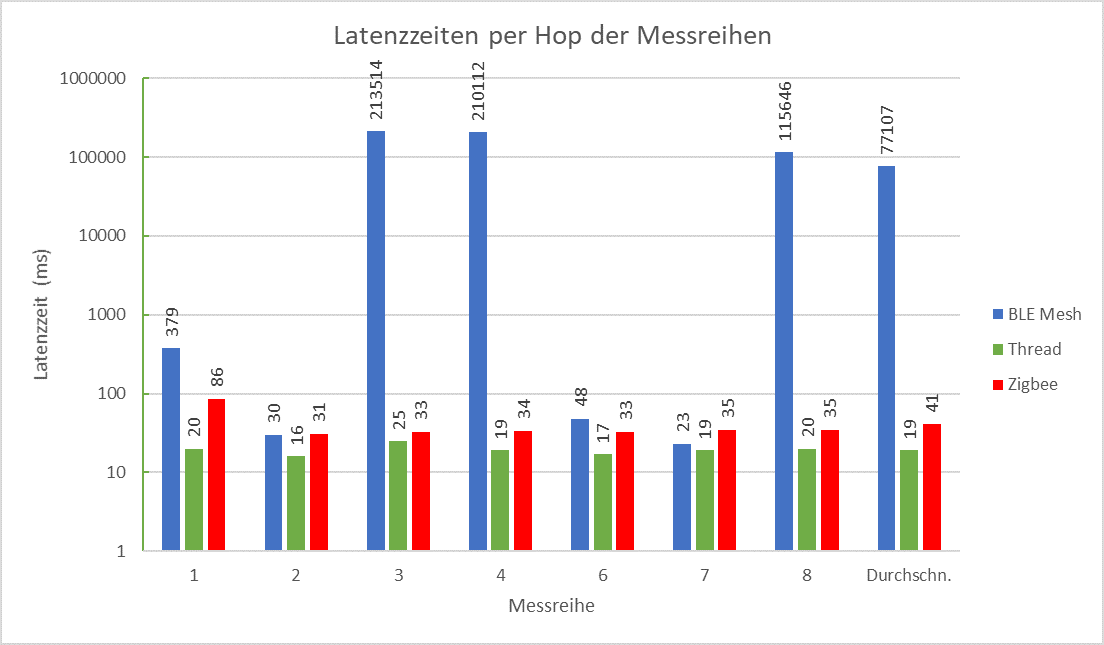
\includegraphics[width=1.0\textwidth]{Latenzzeiten_per_Hop_Messreihen.png}
	\caption{Durchschnittliche Latenzzeit per Hop der einzelnen Messreihen im Vergleich}\label{fig:Latenzzeiten_per_Hop_Messreihen}
\end{figure}

\subsubsection{Durchsatz}\label{subsec:VergleichDurchsatzMessreihen}


\begin{figure}[H]
	\centering
	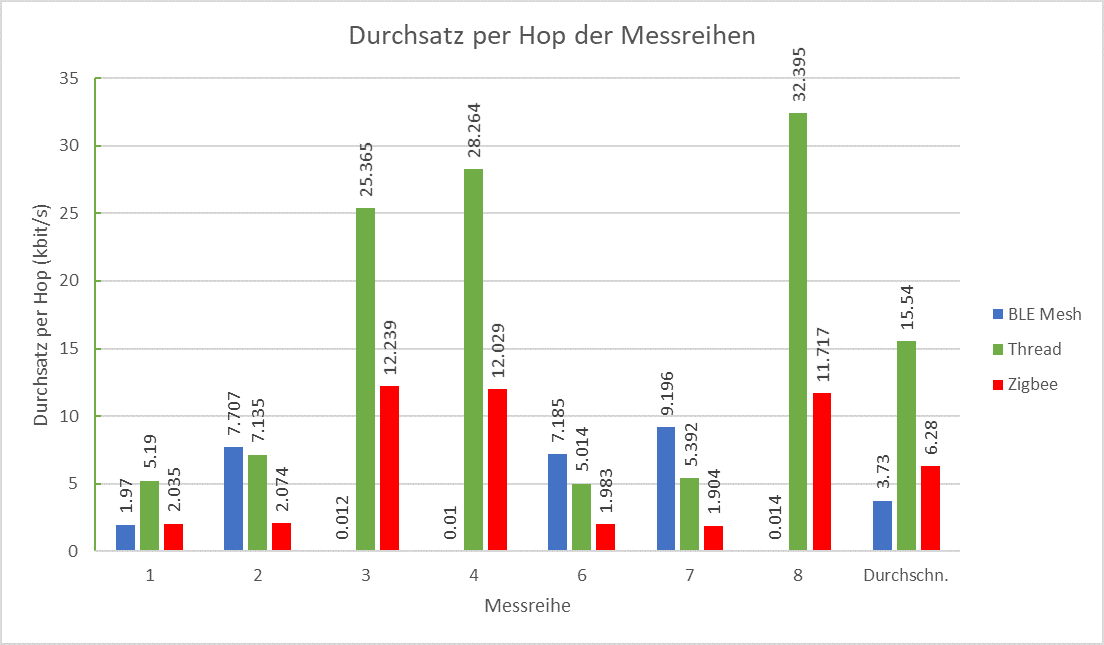
\includegraphics[width=1.0\textwidth]{Durchsatz_per_Hop_Messreihen.png}
	\caption{Durchschnittlicher Durchsatz per Hop der einzelnen Messreihen im Vergleich}\label{fig:Durchsätze_per_Hop_Messreihen}
\end{figure}

\subsubsection{Paketverlust}\label{subsec:VergleichPaketverlustMessreihen}


\begin{figure}[H]
	\centering
	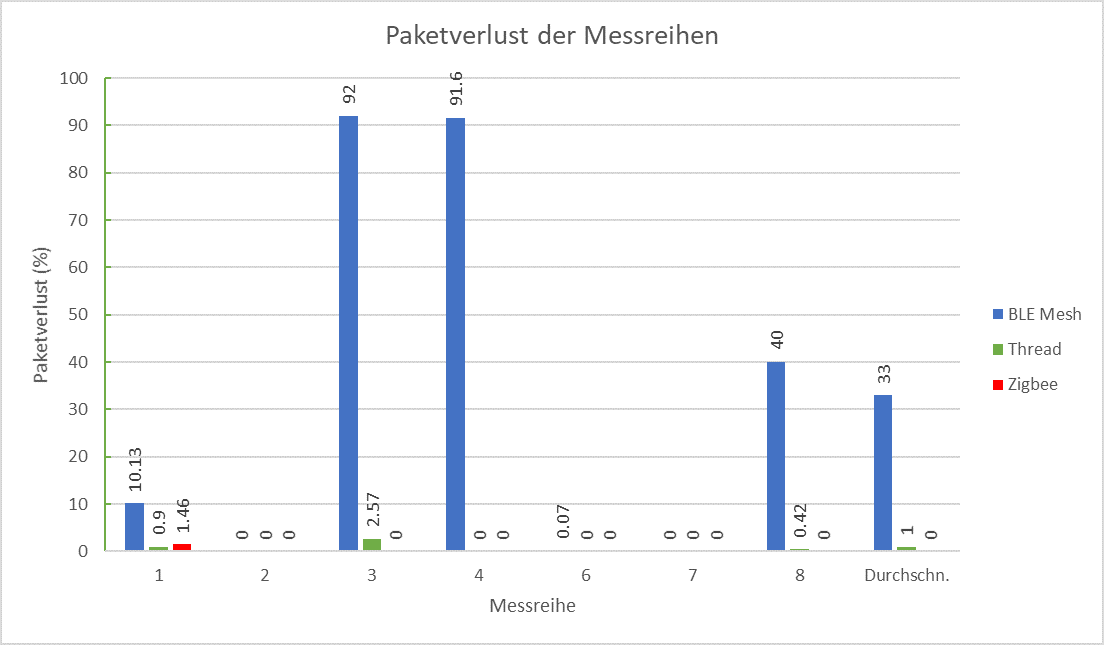
\includegraphics[width=1.0\textwidth]{Paketverlust_Messreihen.png}
	\caption{Durchschnittlicher Paketverlust der einzelnen Messreihen im Vergleich}\label{fig:PaketverlusteMessreihen}
\end{figure}

\subsubsection{Energieverbrauch}\label{subsec:VergleichEnergieverbrauchMessreihen}


\begin{figure}[H]
	\centering
	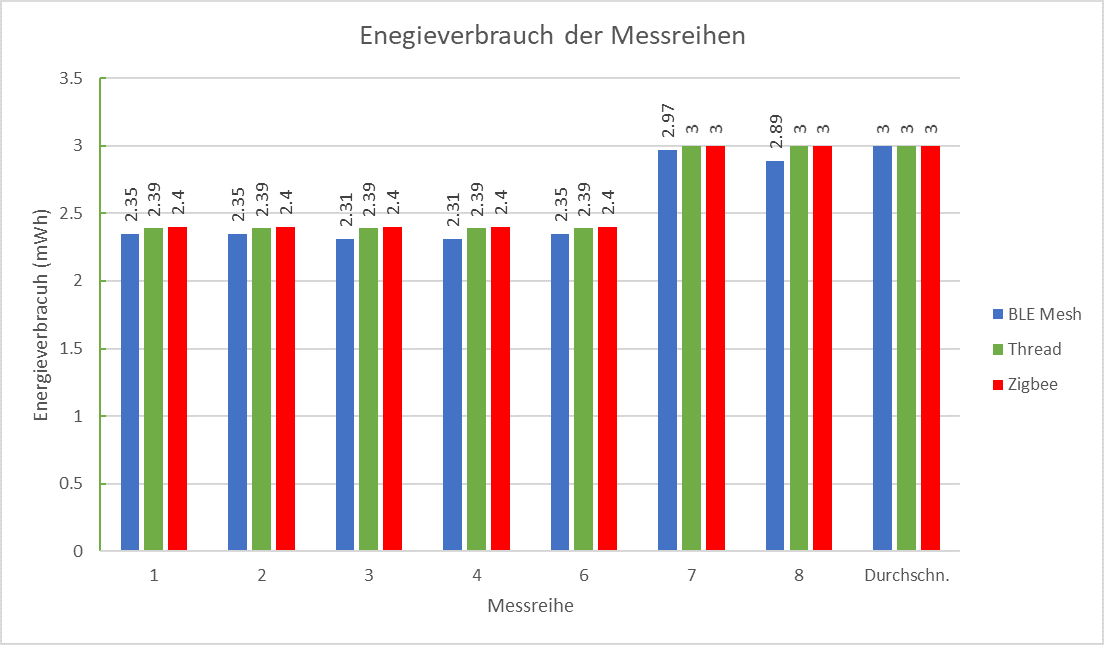
\includegraphics[width=1.0\textwidth]{Energieverbrauch_Messreihen.png}
	\caption{Durchschnittlicher Energiebedarf der einzelnen Messreihen im Vergleich}\label{fig:PaketverlusteMessreihen}
\end{figure}



\subsection{Vergleich Testumgebungen}\label{subsec:VergleichTestumgebungen}

Mithilfe der Unterschiedlichen Testumgebungen wird e

\todo[inline]{Vergleich der drei Netze anhand von spezifischen Merkmalen. Welches Protokoll ist für welche Anwendung geeignet? Wo ist welches Protokoll nicht geeignet?}


\subsubsection{Latenzzeit}\label{subsec:VergleichLatenzzeitTestumgebungen}


\begin{figure}[H]
	\centering
	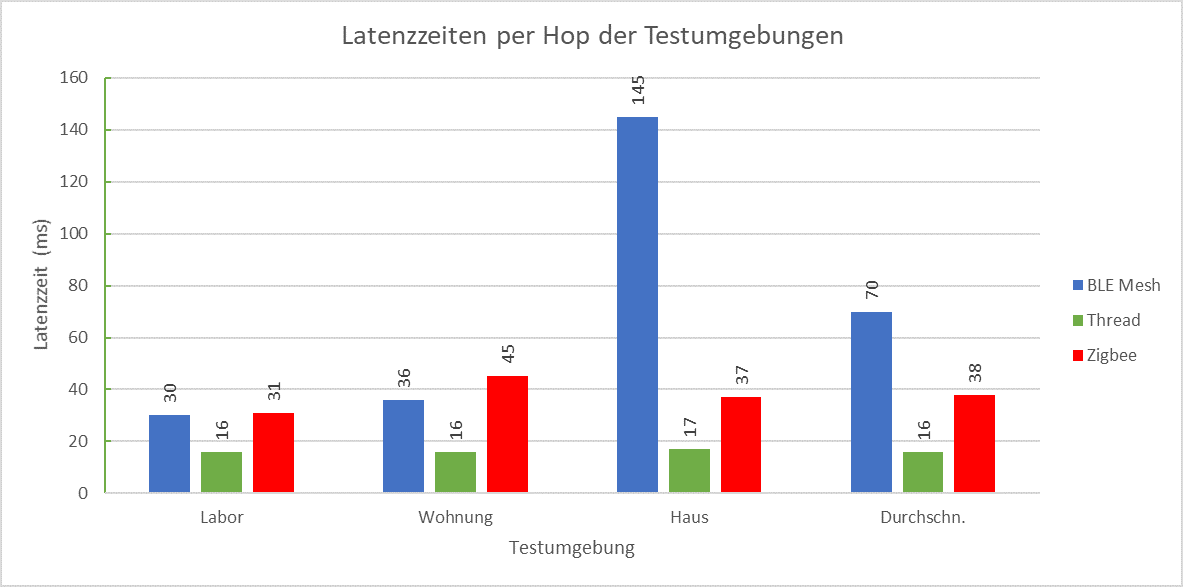
\includegraphics[width=1.0\textwidth]{Latenzzeiten_per_Hop_Testumgebungen.png}
	\caption{Durchschnittliche Latenzzeit per Hop der einzelnen Testumgebungen im Vergleich}\label{fig:Latenzzeiten_per_Hop_Testumgebungen}
\end{figure}

\subsubsection{Durchsatz}\label{subsec:VergleichDurchsatzTestumgebungen}


\begin{figure}[H]
	\centering
	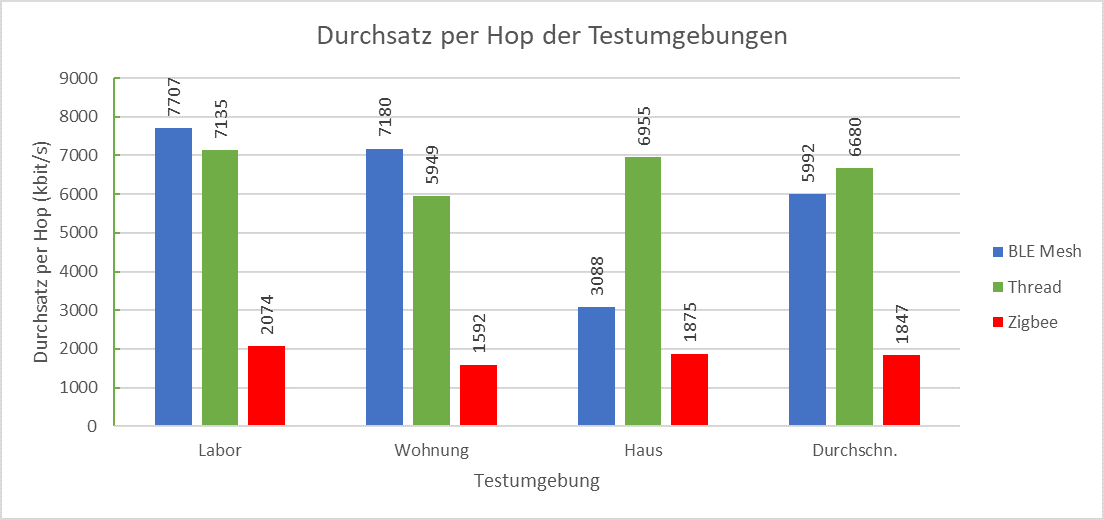
\includegraphics[width=1.0\textwidth]{Durchsatz_per_Hop_Testumgebungen.png}
	\caption{Durchschnittlicher Durchsatz per Hop der einzelnen Testumgebungen im Vergleich}\label{fig:Durchsätze_per_Hop_Testumgebungen}
\end{figure}

\subsubsection{Paketverlust}\label{subsec:VergleichPaketverlustTestumgebungen}


\begin{figure}[H]
	\centering
	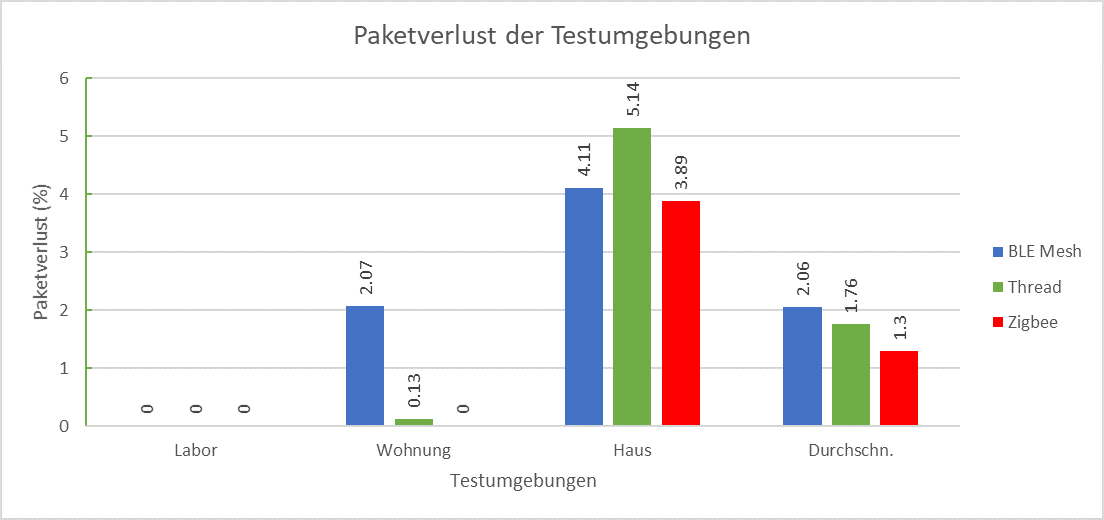
\includegraphics[width=1.0\textwidth]{Paketverlust_Testumgebungen.png}
	\caption{Durchschnittlicher Paketverlust der einzelnen Testumgebungen im Vergleich}\label{fig:PaketverlusteTestumgebungen}
\end{figure}



\subsection{Fazit}\label{subsec:Fazit}
\todo[inline]{Finale Interpretation der Resultate. Welches Protokoll ist das Beste?}

\todo[inline]{Pro / COntra eigene Einschätzung des Stacks... z.B. Thread optimal für Homeautomation.. eher nicht geeiget für Smart Agriculture}

\subsection{Thread}\label{subsec:Thread}

\todo[inline]{Rouben}

\subsection{Zigbee}\label{subsec:Zigbee}

\todo[inline]{Cyrill}

\subsection{Bluetooth Mesh}\label{subsec:Bluetooth_Mesh}

\todo[inline]{Raffi}






